\documentclass{beamer}

% You can also use a 16:9 aspect ratio:
%\documentclass[aspectratio=169]{beamer}
\usetheme{TACC16}
\usepackage{graphicx}

% It's possible to move the footer to the right:
%\usetheme[rightfooter]{TACC16}


% Detailed knowledge of application workload characteristics can
% optimize performance of current and future systems. This may sound
% daunting, with many HPC data centers hosting over 2,000 users running
% thousands of applications and millions of jobs per month.  XALT is an
% open source tool developed at the Texas Advanced Computing Center
% (TACC) that collects system usage information to quantitatively report
% how users are using your system. This session will explore the
% benefits of detailed application workload profiling and how the XALT
% tool has helped leading supercomputing sites unlock the power of their
% application usage data.

%% page 
%\begin{frame}{}
%  \begin{itemize}
%    \item
%  \end{itemize}
%\end{frame}
%
%% page 
%\begin{frame}[fragile]
%    \frametitle{}
% {\tiny
%    \begin{semiverbatim}
%    \end{semiverbatim}
%}
%  \begin{itemize}
%    \item
%  \end{itemize}
%
%\end{frame}



\begin{document}
\title[XALT]{XALT: Job-Level Usage Data on Today's Supercomputers}
\author{Robert McLay}
\date{November 20, 2024}

% page 1
\frame{\titlepage}

% page 2
\begin{frame}{XALT: Outline}
  \center{
\includegraphics[width=.9\textwidth]{XALT_Sticker.png}}
  \begin{itemize}
    \item What is XALT and what it is not?
    \item How it works.
    \item Container issues
    \item Conclusions
    \item This talk: 
  \end{itemize}
\end{frame}

%page 3
\begin{frame}{Understanding what your users are doing}
  \begin{itemize}
    \item Current Version: XALT 3.1.1 (3.2 is coming)
    \item What programs, libraries are your users using?
    \item What imports from R, MATLAB, Python?
    \item What are the top programs by core-hours? by counts? by users?
    \item System, User or Built by Other executables?
    \item Are Executables implemented in C/C++/Fortran/Others?
    \item Track MPI task and/or Threading (\$OMP\_NUMTHREADS)
    \item Function Tracking
    \item Census Taker, Not a performance tool!
  \end{itemize}
\end{frame}

% page 4
\begin{frame}[fragile]
    \frametitle{How XALT 2 works}
 {\tiny
    \begin{semiverbatim}
#include <stdio.h>
void myinit(int argc, char **argv)
\{ printf("This is run before main()\textbackslash{}n"); \}
void myfini()
\{ printf("This is run after main()\textbackslash{}n"); \}

__attribute__((section(".init_array"))) __typeof__(myinit) *__init = myinit;
__attribute__((section(".fini_array"))) __typeof__(myfini) *__fini = myfini;
    \end{semiverbatim}
}
\end{frame}

% page 5
\begin{frame}[fragile]
    \frametitle{How XALT works (III)}
 {\small
    \begin{semiverbatim}
\$ ./try

Hello World!

\$ LD\_PRELOAD=./libxalt.so  ./try
This is run before main()
Hello World!
This is run after main()
    \end{semiverbatim}
}
\end{frame}

% page 6
\begin{frame}{Implications of tracking everything}
  \begin{itemize}
    \item Too much data!! $\Rightarrow$ Sampling
    \item Being in the same namespace of your program
    \item Sharing memory allocation with your program.
    \item Feeling like I'm a developer on every program team.
    \item Fixing these issues has been part of XALT becoming mature.
  \end{itemize}
\end{frame}

% page 7
\begin{frame}{Containers}
  \begin{itemize}
    \item XALT can track executions in Containers
    \item But XALT depends on newer libc than container
    \item When linking libxalt.so to container exec complains
    \item Not sure how to solve this
  \end{itemize}
\end{frame}

% page 8
\begin{frame}{UUID v7}
  \begin{itemize}
    \item XALT uses UUIDs extensively (Univeral Unique ID)
    \item It has used UUID v4 which isn't time sortable
    \item Version 7 is new and \emph{IS} time sortable
    \item This leads to faster indexing in a database
    \item XALT 3.1.1+ now uses UUIDv7 on computers that support
      getentropy function in libc
  \end{itemize}
\end{frame}

% page 9
\begin{frame}{Updating Python $<=>$ MySQL interface}
  \begin{itemize}
    \item XALT has used MySQLdb as its interface.
    \item This package is nolonger supported.
    \item XALT is switching to mysql.connector.python 
  \end{itemize}
\end{frame}



% page 10
\begin{frame}[fragile]
    \frametitle{XALT Doc usage by City}
    \center{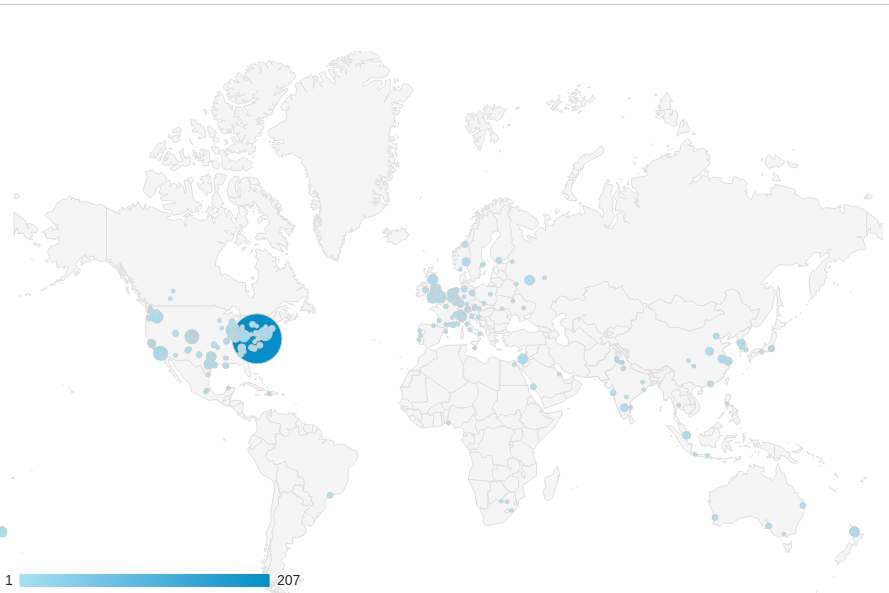
\includegraphics[width=.9\textwidth]{XALT_doc_usage_by_city}}
\end{frame}

% page 11
\begin{frame}{XALT Monthly Zoom Mtg}
  \begin{itemize}
    \item Usually the 3rd Thursday of the Month at 10:00 am US Central
    \item Feel free to attend when you have questions or concerns and
      not when you don't.
  \end{itemize}
\end{frame}

% page 11
\begin{frame}{Conclusions}
  \begin{itemize}
    \item XALT is useful and low cost tool to know how your users run
      on your system.
  \end{itemize}
\end{frame}

%
\begin{frame}{License}
\footnotesize
\textcopyright The University of Texas at Austin, \the\year\\
\vspace{0.5 cm}
This work is licensed under the Creative Commons Attribution Non-Commercial 3.0 Unported License. To view a copy of this license, 
visit http://creativecommons.org/licenses/by-nc/3.0/\\
\vspace{0.5 cm}
When attributing this work, please use the following text: 
"Designing and Administering Large-scale Systems", Texas Advanced Computing Center, \the\year. Available under a Creative Commons Attribution Non-Commercial 3.0 Unported License.
\newline
\newline

\includegraphics[width=1cm]{./figures/cc.png}
\end{frame}

\end{document}

% t2308150115
